\section {Gestione dati raccolti}
Tutti i meccanismi per rilevare intrusioni sono stati implementati per produrre due tipi di informazioni:
\begin{enumerate}
  \item Determinare qualora vi sia stata un'intrusione
  \item Fornire dati all'utente dell'avvenuta intrusione
\end{enumerate}
Ovviamente se tali dati rimanessero localizzati al dispositivo che li ha prodotti verrebbe meno l'utilità stessa dell'applicazione. Si è quindi reso necessario un meccanismo di notifica all'utente:
\begin{enumerate}
  \item L'utente viene avvisato dell'avvenuta intrusione
  \item I dati vengono spediti ad un server dedicato di modo da poter essere consultati dall'utente in qualsiasi momento
\end{enumerate}
Tali operazioni sono naturalmente subordinate alle preferenze specificate dall'utente nella schermata principale dell'applicazione e alle effettive risorse disponibili al dispositivo (ad esempio non è possibile inviare i dati al server se il dispositivo non ha accesso alla rete, come non è possibile mandare un SMS di allerta qualora non vi sia copertura telefonica).\\
Tutta l'applicazione verte quindi sulla generazione, elaborazione e memorizzazione di dati:
\begin{enumerate}
  \item A seconda delle impostazioni abilitate dall'utente, il dispositivo inizia a monitorare l'ambiente producendo dati. Durante questa fase vengono prodotti dati grezzi che non hanno alcun significato per l'applicazione
  \item I dati raccolti dall'ambiente vengono elaborati a seconda della loro tipologia. Durante questa fase i dati grezzi vengono elaborati per fornire informazioni statistiche alle quali l'applicazione è in grado di associare, in un secondo momento, un significato.\\
  \textit{Poiché tali elaborazioni possono essere particolarmente onerose, vengono creati degli appositi daemon in grado di effettuare le computazioni necessarie, di modo da non sovraccaricare il thread grafico e mantenerlo quindi responsivo}
  \item I dati elaborati o le informazioni da loro ricavate vengono confrontate con valori di soglia (sensibilità impostate dall'utente) per stabilire se è necessario generare un allarme. Durante questa fase le informazioni statistiche prodotte durante la fase precedente vengono trasformate in informazioni semantiche per l'applicazione (informazioni semantiche basilari: c'è stata intrusione/non c'è stata intrusione)
  \item Qualora sia necessario generare un allarme vengono utilizzate tutte le risorse disponibili (conformemente alle preferenze specificate) per notificare l'utente dello stato anomalo che è stato registrato dal dispositivo
  \item Vengono spediti in un luogo sicuro (il server predisposto) tutti i dati in possesso all'applicazione. I dati inviati sono sostanzialmente (a meno di conversioni di formato) i dati grezzi catturati dal dispositivo durante la prima fase. Da notare che questi dati, nonostante non abbiano alcun significato per l'applicazione stessa, assumono una valenza semantica per l'utente, in quanto sono dati comprensibili e significativi per un essere umano (coordinate, audio, immagini)
\end{enumerate}
Qualora uno qualsiasi dei tre meccanismi predisposti al monitoraggio dell'ambiente riconosca uno stato anomalo, l'applicazione si preoccupa di inviare tutti i dati da lei posseduti.

\subsection{Allerta tramite SMS}
Il più semplice sistema di notifica è quello di inviare un SMS al numero specificato dall'utente tramite la schermata principale dell'applicazione.\\
L'informazione contenuta nel messaggio è basilare e serve semplicemente per segnalare che l'applicazione ha riscontrato uno stato anomalo dell'ambiente sorvegliato. Questo messaggio segnala implicitamente che è possibile ottenere informazioni più accurate consultando il server al quale l'applicazione ha inviato i dati (qualora l'utente abbia abilitato le opzioni necessarie).

\subsection{Utilizzo della rete}
Qualora il dispositivo abbia accesso alla rete, l'applicazione si preoccupa di inviare al server predisposto tutte le informazioni accumulate.\\
Le informazioni che l'applicazione tenta di memorizzare sul server di modo da essere accedute dall'utente in qualsiasi momento sono di tre tipi:
\begin{enumerate}
  \item Immagini catturate dalla fotocamera. Poiché le immagini sono informazioni particolarmente onerose da inviare, è stato deciso di inviare un differente numero di immagini a seconda della tipologia di collegamento disponibile: tutte le immagini catturate qualora si sia connessi tramite WiFi, solo metà qualora si sia connessi tramite 3G
  \item Audio catturato dal microfono. Viene inviato (indifferentemente dal tipo di collegamento disponibile) un file audio contenente 10 secondi di registrazione
  \item Coordinate della posizione del dispositivo. Questo tipo di informazione, una volta sollevato l'allarme, viene spedito periodicamente al server di modo da poter tracciare il possibile spostamento del dispositivo (e quindi del malfattore). Per ottenere questa informazione è possibile utilizzare il GPS qualora sia attivo o sfruttare meccanismi di geo-localizzazione disponibili in rete
\end{enumerate}

\begin{figure}[!ht]
\begin{center}
\makebox[\linewidth]{
\subfigure[Schermata nella quale è possibile visualizzare l'ultima posizione conosciuta del dispositivo]{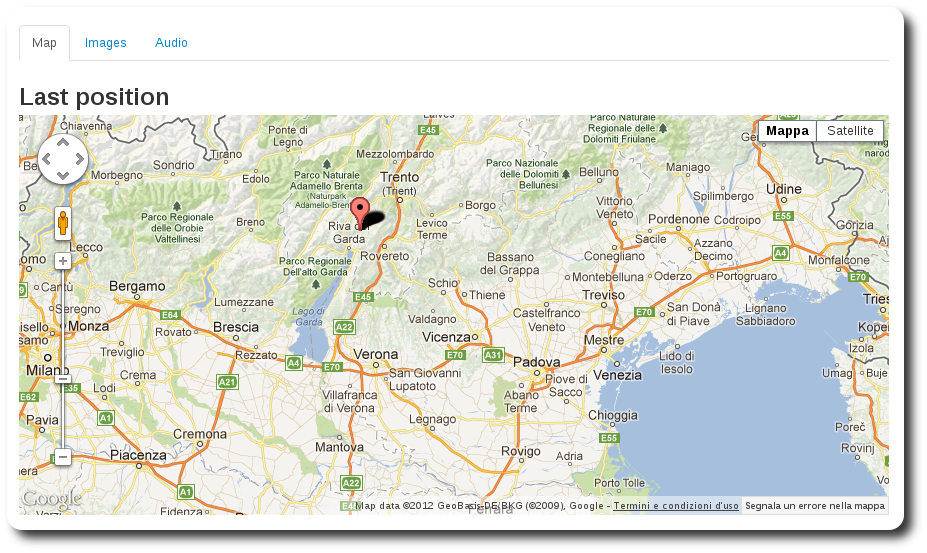
\includegraphics[scale=.3]{./../wireless/resources/map.png}}~
\subfigure[Schermata nella quale è possibile visualizzare le foto scattate dalla fotocamera]{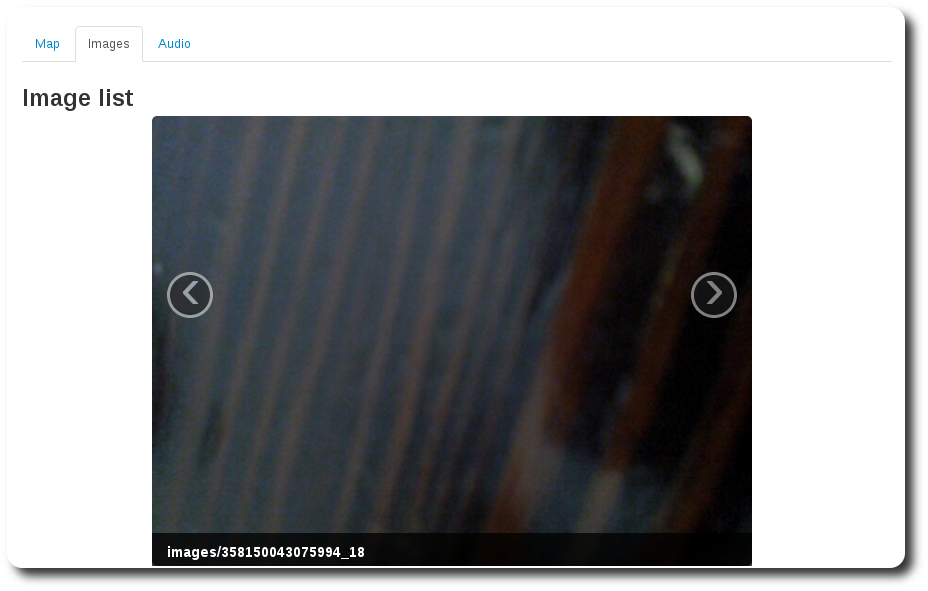
\includegraphics[scale=.3]{./../wireless/resources/slideshow.png}}}
\end{center}
\caption{Visualizzazione delle informazioni spedite al server}
\label{fig:informazioniServer}
\end{figure}

Per spedire le informazioni al server vengono utilizzate le API REST messe a disposizione dal server:
\begin{lstlisting}[caption=API REST utilizzate per spedire dati al server]
[POST]	/api/phones/:phoneId/images
[POST] 	/api/phones/:phoneId/audio
[POST]  /api/phones/:phoneId/positions
\end{lstlisting}
Per poter utilizzare tali API è però necessario accertarsi dell'identità del dispositivo che tenta di inviare le informazioni. \`E quindi stata predisposta un'ulteriore API REST utilizzabile per ottenere un \textit{access token}:
\begin{lstlisting}[caption=API REST utilizzate per identificarsi e ricevere l'access token]
[POST]	/users/accesstoken
\end{lstlisting}
Tale token investe il dispositivo dell'autorità di poter eseguire l'upload di informazioni in quanto, per poter ricevere e quindi avere a disposizione tale token, è necessario essere in possesso delle corrette credenziali con le quali l'utente (e quindi il dispositivo) è noto al server (credenziali spedite in POST assieme alla richiesta per l'\textit{access token}).

\subsection{Utilizzo bluetooth}
Qualora non si abbia accesso alla rete ed il bluetooth sia attivo, il dispositivo tenterà di mettersi in collegamento con altri dispositivi (che abbiano installata la stessa applicazione) per demandare a loro il compito di inviare dei dati al server. Poiché sarebbe troppo oneroso eseguire uno scambio di immagini e file audio, l'unica informazione che si richiede ad altri dispositivi di spedire al server è l'informazione riguardante la locazione del dispositivo al momento del collegamento.\\
Per poter raggiungere questo obiettivo è necessario:
\begin{itemize}
  \item Che le informazioni inviate al server non siano fasulle: ossia è necessario assicurarsi che i dati spediti da un dispositivo per conto di un altro siano informazioni veritiere e che non sia possibile contraffarle
  \item Che non vi sia la necessità di richiedere all'utente l'abilitazione di creare un collegamento bluetooth: non è plausibile che l'utente del dispositivo a cui si sta tentando di chiedere aiuto controlli in continuazione il proprio dispositivo per l'evenienza che vi sia un dispositivo rubato che tenta di collegarsi
\end{itemize}

Il primo requisito viene soddisfatto applicando un piccolo protocollo di firma dei dati ispirato al protocollo Kerberos. Chiamando ``dispositivo delegato'' il dispositivo a cui si richiede di inviare le informazioni al server e ``dispositivo richiedente'' il dispositivo che vuole inviare al server i propri dati ma che non può considerata l'assenza di rete, il protocollo che si è implementato (schematizzato in figura \ref{fig:protocolloBluetooth}) è:
\begin{enumerate}
  \item Il dispositivo richiedente invia un \texttt{HelloMessage} ai dispositivi verso i quali è riuscito ad aprire una connessione (ossia i potenziali dispositivi delegati). All'interno di questo messaggio l'unica informazione importante è l'identificativo del dispositivo richiedente, identificativo che verrà usato dal dispositivo delegato per sapere dove inviare le informazioni (in quanto le API REST sono indicizzare sull'identificativo dei dispositivi)
  \item Il dispositivo delegato risponde con un \texttt{KeyRequest}, all'interno del quale si trovano le informazioni riguardanti latitudine e longitudine.
  \item Il dispositivo richiedente utilizza l'algoritmo AES per cifrare le informazioni contenute all'interno di \texttt{KeyRequest} ed ottenere così l'\texttt{authorization\_key}. L'\texttt{authorization\_key} viene quindi rispedita al dispositivo delegato all'interno di un \texttt{KeyResponse}
  \item Il dispositivo delegato invia quindi al server le informazioni di latitudine, longitudine e \texttt{authorization\_key} utilizzando l'API REST \texttt{[POST] /api/phones/:phoneId/position/delegated}
  \item Il server decifrando \texttt{authorization\_key} è in grado di determinare se il dispositivo delegato era veramente autorizzato a richiedere la memorizzazione dei dati
\end{enumerate}
\begin{figure}[!ht]
\begin{center}
\makebox[\linewidth]{\securityProtocol}
\end{center}
\caption{Schema del protocollo per l'autenticazione dei dati inviati al server da un dispositivo delegato.}
\label{fig:protocolloBluetooth}
\end{figure}
Ovviamente questo protocollo può funzionare solamente se la chiave di cifratura (e quindi di decifratura in quanto AES è un algoritmo di cifratura simmetrico) è condivisa solo ed esclusivamente tra server e dispositivo richiedente. Infatti questo protocollo si basa sul fatto che solo il dispositivo che ha la chiave corretta è in grado di cifrare il messaggio che viene spedito al server: al server non basterà che controllare che il messaggio decifrato sia identico alle informazioni spedite in chiaro dal dispositivo delegato.\\
La chiave che viene utilizzata all'interno di AES è una speciale sequenza alfanumerica condivisa esclusivamente tra server e dispositivo: il protocollo offre quindi la possibilità di stabilire l'autorità di un certo dispositivo ad inserire informazioni in vece di un altro dispositivo.\\

Il secondo requisito viene soddisfatto sfruttando un particolare tipo di bluetooth server socket offerto dalle API Android: \texttt{listen\-Using\-Insecure\-Rfcomm\-With\-Service\-Record}. Nonostante venga sconsigliato utilizzare questo tipo di socket, in quanto non richiedendo l'esplicito consenso dell'utente può essere utilizzato per nuocere al dispositivo, è proprio il tipo di socket che permette il tipo di connessione di cui l'applicazione necessita.

